\documentclass[11pt,a4paper]{article}

\usepackage[margin=2.1cm]{geometry}
\usepackage[T1]{fontenc}
\usepackage{lmodern}
\usepackage{amsmath,amssymb}
\usepackage{booktabs}
\usepackage{graphicx}
\usepackage{caption}
\usepackage[round]{natbib}
\usepackage[hidelinks]{hyperref}
\usepackage{enumitem}
\usepackage{xcolor}

\graphicspath{{figures/}}
\captionsetup{font=small,labelfont=bf}
\setlist{nosep,leftmargin=*}
\setlength{\parskip}{3pt}

% Notebook reference, e.g. \nb{02}
\newcommand{\nb}[1]{\textcolor{gray}{\small[\texttt{notebooks/#1}]}}

\title{\vspace{-1.2cm}Trading the Corn--Soybean Spread:\\ Cointegration, Machine Learning and Regime Switching}
\author{Roos de Brabander \and Wiktor Grocholewski \and Antonio Harley \and Artem Zeziulin\\[2pt]
\small Trading and Investment Club, Spring 2026}
\date{\small September 2026}

\begin{document}
\maketitle
\vspace{-0.6cm}

\begin{abstract}
\noindent
Corn and soybean compete for the same farmland and respond to the same demand and weather shocks, so a hedged
position in the two should mean-revert. We test this idea with models of increasing complexity: z-score rules on the
cointegrated pair and on baskets including wheat and cotton, a portfolio of pairs with Ornstein--Uhlenbeck-based
capital allocation, a triple-barrier machine-learning classifier with weather features, and a Bayesian regime-switching
model in which weather drives the regime. With every parameter chosen on training data and P\&L measured as
tradeable, capital-normalised returns, no strategy achieves an out-of-sample Sharpe ratio that is statistically
distinguishable from zero. The most useful output of the project is a set of lessons on how easily a backtest of a
slow, persistent spread overstates performance.
\end{abstract}

%=====================================================================
\section{Introduction}
%=====================================================================
Corn and soybean prices move together: farmers rotate the two crops on the same land and both are driven by feed
and energy demand. If the two are \emph{cointegrated}, a suitably hedged spread is stationary and can be bought when it is
unusually low and sold when it is unusually high \citep{chan2013}. A second idea was that weather in the main
growing regions (the US Corn Belt and Brazil) moves the relative supply of the two crops and could help to time
such trades.

The report follows the project from the simplest to the most complex model; each section corresponds to a notebook
of the accompanying code, shown as \nb{0x} (functions in \texttt{src/}): data \nb{01}, the corn--soybean pair
\nb{02}, wheat and cotton \nb{03}, machine learning \nb{04, 05} and regime switching \nb{06}.
Section~\ref{sec:lessons} summarises the results and what we learned.

\paragraph{Common conventions.} Strategies hold $+1$, $0$ or $-1$ units of a spread (the ML strategies may also size
by predicted probability). The hedge (units of each
asset per unit of spread) is \emph{frozen} when a trade is opened: letting a rolling hedge ratio drift inside a trade
produces P\&L that could only be earned by re-hedging every day \citep[\S2.4]{lopezdeprado2018}. Daily returns are P\&L
divided by the gross capital committed at entry, $\sum_i |u_i| P_{i,t_0}$, and Sharpe ratios are annualised with a zero
risk-free rate. Every threshold, window and hyperparameter is chosen on a training sample and evaluated once on a later
test sample.

%=====================================================================
\section{Data}\label{sec:data}
%=====================================================================
\textbf{Prices.} We use two price sources from Yahoo Finance. Front-month \emph{futures} (ZC=F, ZS=F) cover
2005--2026, but the continuous series jumps at every contract roll; we realised this after the first strategies were
built on it. From then on we used commodity \emph{ETFs}, which roll internally: Teucrium CORN, SOYB and WEAT and the
WisdomTree cotton ETC COTN (available from 2011; the originally used iPath BAL was delisted in 2023). Section~\ref{sec:pair}
still uses futures because of their longer history; its results carry this caveat.

\textbf{Weather.} Daily weather from the Open-Meteo archive for three locations in each growing region: the US Corn
Belt and southern/central Brazil (corn and soybean), the US wheat belt, and China and India (cotton). For each location
we keep 15 crop-stress variables (temperature, precipitation, soil moisture, evapotranspiration, humidity, wind\ldots)
and form 30-day backward-looking aggregates: sums for precipitation, minima for soil moisture, maxima for wind and means
otherwise. Weather is forward-filled onto trading days, so every day only sees past weather.

\textbf{Samples.} Sections~\ref{sec:pair}--\ref{sec:multi} split each sample chronologically into 70\% training and
30\% test. The machine-learning sections keep the last 375 labelled observations ($\approx$1.5 years) as a holdout
and use walk-forward cross-validation on the rest.

%=====================================================================
\section{The corn--soybean pair}\label{sec:pair}
%=====================================================================
\begin{table}[t]
\centering\small
\caption{Out-of-sample performance of all strategies (annualised; returns on capital; no transaction costs). Train =
training sample (Sections 3--4) or walk-forward CV (Section 5); every parameter was chosen on it. Test years: 6.3
(Section 3), 4.4 (Section 4), 1.5--1.7 (Section 5). Full tables in \texttt{report/tables/}.}
\label{tab:results}
\begin{tabular}{llrrrr}
\toprule
& Strategy & Train SR & Test SR & Test return p.a. & Test max DD \\
\midrule
\multicolumn{6}{l}{\emph{Corn--soybean futures, test Oct 2019--Feb 2026} \nb{02}}\\
A  & price levels, rolling OLS          & $-0.01$ & $-0.27$ & $-1.3\%$ & $-24\%$ \\
B1 & log prices, static Johansen        & $0.16$  & $0.58$  & $6.1\%$  & $-14\%$ \\
B2 & log prices, Kalman                 & $0.64$  & $0.01$  & $0.1\%$  & $-22\%$ \\
B3 & log prices, rolling Johansen       & $0.40$  & $0.10$  & $1.0\%$  & $-20\%$ \\
\midrule
\multicolumn{6}{l}{\emph{Soybean, corn, wheat, cotton ETFs, test Nov 2021--Apr 2026} \nb{03}}\\
C  & rolling Johansen, 4 commodities    & $0.95$  & $0.35$  & $2.8\%$  & $-12\%$ \\
C  & rolling Johansen, four 3-commodity baskets & 0.14 to 0.98 & $-0.65$ to $0.15$ & & \\
D  & 4 commodities in logs (static / Kalman / rolling) & 0.63 to 0.81 & $-0.28$ to $-0.03$ & & \\
E  & pairs portfolio, equal weight      & $0.38$  & $0.42$  & $3.5\%$  & $-15\%$ \\
E  & pairs portfolio, MRB               & $0.07$  & $0.38$  & $3.2\%$  & $-16\%$ \\
E  & pairs portfolio, MRR               & $0.24$  & $0.46$  & $3.7\%$  & $-15\%$ \\
\midrule
\multicolumn{6}{l}{\emph{Machine learning, holdout of 375 labelled days, Dec 2023--Sep 2025} \nb{04, 05}}\\
ML & XGBoost corn--soybean, probability sizing & CV acc.\ 55\% & $0.76$ & $2.4\%$ & $-3\%$ \\
ML & XGBoost corn--soybean, sign sizing & CV acc.\ 55\% & $0.41$ & $3.0\%$ & $-5\%$ \\
ML & six-pair portfolio, EW / MRB / MRR & -- & 0.51 / 0.68 / 0.66 & 1.3--2.9\% & $-3$ to $-4\%$ \\
\bottomrule
\end{tabular}
\end{table}

\textbf{Tests} \nb{02}. On the training sample (2005--2019) both prices are I(1). The evidence for cointegration is
weaker than it first appeared: with the correct residual-based critical values the Engle--Granger test
\citep{englegranger1987} does \emph{not} reject the null of no cointegration for price levels ($t=-2.88$,
$p=0.14$)\footnote{The first version of the project used ordinary ADF $p$-values on the estimated residual, which gave
$p=0.003$.}, while the Johansen trace test \citep{johansen1991} on log prices rejects at 1\% (trace 25.1 vs.\ 19.9).
In an error-correction model soybean is pulled back towards the long-run relation ($\gamma=-0.008$, $p<0.001$), but
slowly: the half-life of the spread is 84 trading days in levels and 98 in logs, and after the training sample the
static spread drifts away from zero.

\textbf{Strategies.} All strategies enter when the z-score of the spread relative to its trailing mean exceeds a
threshold and exit when it crosses zero.
\begin{itemize}
\item[\textbf{A}] \emph{Price levels, rolling OLS.} Soybean is regressed on corn over the previous 252 days; the
spread and its z-score use the same window.
\item[\textbf{B}] \emph{Log prices.} The spread $\log S_t-\beta_t\log C_t-\alpha_t$ is a portfolio of \$1 of soybean
and \$$\beta_t$ of corn, so the hedge is converted from dollars to units before computing P\&L. We compare three
estimators of $\beta_t$: the static Johansen vector (B1), a Kalman filter with random-walk coefficients \citep[ch.~3]{chan2013}
(B2), and a rolling Johansen vector (B3, traded only when yesterday's $|\beta|\le 2$). The z-score window equals the
half-life.
\end{itemize}

\textbf{Results.} Table~\ref{tab:results} (top) and Figure~\ref{fig:pair}. Strategy A loses money in the training
sample for every entry threshold once P\&L is computed with the frozen hedge, and it loses out of sample. Among the
log-price strategies, the most flexible one (Kalman) has the best training Sharpe ratio (0.64) and a test Sharpe of
0.01 --- a textbook case of fitting noise. The static Johansen spread does best out of sample (Sharpe 0.58, +42\% over
six years), but its training Sharpe was only 0.16, and a Sharpe of 0.58 over 6.3 years has a standard error of
about 0.4 \citep{lo2002}: it is the best of four specifications, not evidence of an edge.

\begin{figure}[t]
\centering
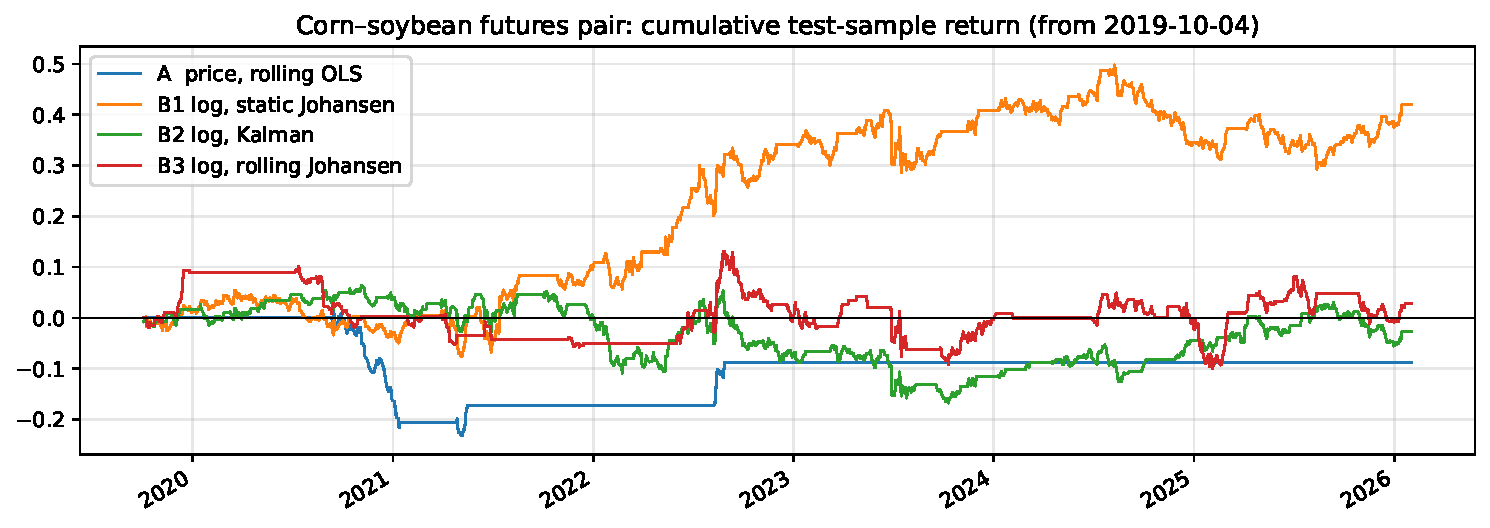
\includegraphics[width=0.9\textwidth]{pair_test_returns.pdf}
\vspace{-0.6cm}
\caption{Corn--soybean futures pair: cumulative test-sample return of the four specifications (2019--2026). \nb{02}}
\label{fig:pair}
\end{figure}

%=====================================================================
\section{More commodities: baskets and a portfolio of pairs}\label{sec:multi}
%=====================================================================
A single spread is exposed to breakdowns of one relation, so we added wheat and cotton (ETFs, 2011--2026) \nb{03}.

\textbf{Cointegrated baskets.} Johansen tests on the training sample (2011--2021) find cointegration at 95\% for three
of the five baskets in price levels (all four commodities; soybean--corn--wheat; corn--wheat--cotton) and for none in
log prices. Where it holds, the half-life of the basket is about 35 days, half that of the pair. We trade every basket
with a rolling (252-day) Johansen eigenvector in price levels (strategy C) and the four-commodity basket in log prices
with the three hedge estimators of Section~\ref{sec:pair} (strategy D). Out of sample the results scatter around zero
(test Sharpe from $-0.65$ to $0.35$), with no relation to the cointegration tests: the two best baskets include one
that fails the test, and all three log-price variants lose money despite training Sharpe ratios of 0.6--0.8.

\textbf{Portfolio of pairs} (strategy E). Following \citet{lee2023}, all six pairs are traded with a z-score rule on a
rolling-OLS spread, and at every rebalancing date capital is re-allocated from an Ornstein--Uhlenbeck fit to each
spread: equal weights (EW), weights $\propto$ normalised reversion speed $\times$ OU log-likelihood (MRB), or fixed
weights by the rank of that score (MRR). All parameters are tuned jointly on the training sample. This is the most
consistent strategy of the project: a test Sharpe of 0.38--0.46 over 4.4 years for all three allocations
(Table~\ref{tab:results}), with a similar training Sharpe for EW. The OU allocation does not improve on equal weights:
all four markets share the same drivers, so the spreads are correlated and the cross-section of OU scores carries
little information. An earlier version reported a Sharpe of 1.6 for this strategy; that number measured P\&L in units
of spread standard deviations rather than capital, and was obtained with parameters tuned on the full sample.

%=====================================================================
\section{Machine learning}\label{sec:ml}
%=====================================================================
\textbf{Set-up} \nb{04}. Instead of a fixed rule, a classifier predicts whether buying the spread \emph{today} ends
in profit, following \citet{lopezdeprado2018} (AFML). The hedge ratio of soybean on corn (ETFs) comes from a 504-day rolling OLS
(labels) and a three-state Kalman filter (features): the usual two-state filter absorbs a temporarily wide spread into
the hedge ratio, so we add the spread as an AR(1) hidden state, $\xi_t=[\alpha_t,\gamma_t,s_t]'$ with transition
$\mathrm{diag}(1,1,\phi)$.
\begin{itemize}
\item \emph{Labels} (AFML ch.~3--4): for an entry on every day, the P\&L of a long-spread position with the hedge
frozen at entry is followed until it reaches $\pm2.5$ daily standard deviations or 200 trading days; the label is its
sign. Labels overlap heavily (mean uniqueness 0.09), so observations are weighted by their average uniqueness.
\item \emph{Features}: four Kalman features (spread level, innovation and two z-scores), spread volatility, month,
weekday and 90 rolling weather variables from the US and Brazil.
\item \emph{Validation} (ch.~7, 11): the last 375 observations (Jan 2024--Jul 2025) are a holdout used once; on the rest
we use walk-forward cross-validation with purging, because symmetric purged $k$-fold would train on later folds whose
rolling-OLS and Kalman features were estimated from test-fold prices.
\item \emph{Selection and models} (ch.~4, 6, 8, 9): union of the top-20 features by MDI and by MDA, minus features with
negative MDA (32 remain); XGBoost and a random forest on sequentially bootstrapped bags; 525 XGBoost and 27 pipeline
configurations tuned by walk-forward log-loss.
\end{itemize}

\textbf{Results.} Weather carries a little information: walk-forward accuracy rises from 50\% with the six non-weather
features to 55\% with weather, and the log-loss (0.671) is slightly below that of a coin flip ($\ln2=0.693$). The signal
is unstable, however --- the first fold (2017--2020) has an accuracy below 50\% --- and hyperparameter tuning adds
nothing. On the holdout XGBoost is right 60\% of the time but has a log-loss of 0.718, worse than a coin flip: its
probabilities are over-confident. The random forest (51\%) does not beat always predicting the majority class (53\%).
Traded on the holdout, the signal earns Sharpe ratios of 0.3--0.8 depending on sizing and rebalancing, but over 1.5
years the standard error is about 0.9, the strategy is net long soybean, and the result is fragile: purging four
observations at the dev/holdout boundary moved the Sharpe ratios by about 0.2.

\textbf{Six pairs} \nb{05}. Running the same pipeline for all six pairs, with the weather of each pair's growing
regions, and combining the pairs with the OU allocation of Section~\ref{sec:multi} gives holdout Sharpe ratios of
0.5--0.7 over about 1.7 years (Table~\ref{tab:results}). The gains come from the two soybean pairs with US-grown
partners (corn, wheat); the corn--wheat and corn--cotton models never cross the confidence band ($|p-0.5|>0.15$) and do
not trade, and the pairs with cotton lose. The result is also sensitive to seemingly innocuous choices: before the
clean-up, with corn as the dependent leg and all pairs restricted to the common four-asset calendar, the same analysis
gave Sharpe ratios between $-0.2$ and 0.

%=====================================================================
\section{Bayesian regime switching}\label{sec:regime}
%=====================================================================
Finally we asked whether the spread reverts to \emph{different} equilibria in different growing conditions, with
weather shifting the probability of each regime \nb{06}. The Kalman spread $y_t$ follows
\begin{equation*}
y_t=(1-\phi)\,\mu_{s_t}+\phi\,y_{t-1}+\varepsilon_t,\qquad
z_t=\alpha_0+w_t'\alpha+h_t'\kappa+\delta\,s_{t-1}+\eta_t,\qquad s_t=\mathbb{1}[z_t>0],
\end{equation*}
with $\mu_0<\mu_1$, weather $w_t$, Fourier seasonal terms $h_t$ and persistence $\delta>0$. A Gibbs sampler draws the
state path by forward-filtering backward-sampling \citep{carterkohn1994}, the probit utilities as in
\citet{albertchib1993}, and the remaining parameters from conjugate conditionals.

The sampler does not converge (Geweke statistics far beyond $\pm2$), the regime means have posterior standard
deviations of 1.5--3, and the regime probability merely follows an annual cycle. Two checks explain why. First, with $\phi\approx0.996$ the regime mean enters each observation only as
$(1-\phi)\mu_{s_t}$, far below the noise. Simulating the model with \emph{known} regimes shows the posterior standard
deviation of $\mu$ growing from 0.01 at $\phi=0.5$ to almost 1 at $\phi=0.99$ (Figure~\ref{fig:regime}): the regime
means are not identified at realistic sample sizes. Second, the bimodal histogram of the spread that motivated the
model is an artefact of persistence: 87\% of simulated single-regime AR(1) paths with the same $\phi$ and $\sigma$ also
prefer a two-component Gaussian mixture, and the real data sits at the 87th percentile of that null. Weather adds
almost nothing to an AR(1) for daily spread changes (incremental $R^2$ of 0.4\%, joint $F$-test $p=0.06$). We therefore
did not trade this model.

\begin{figure}[t]
\centering
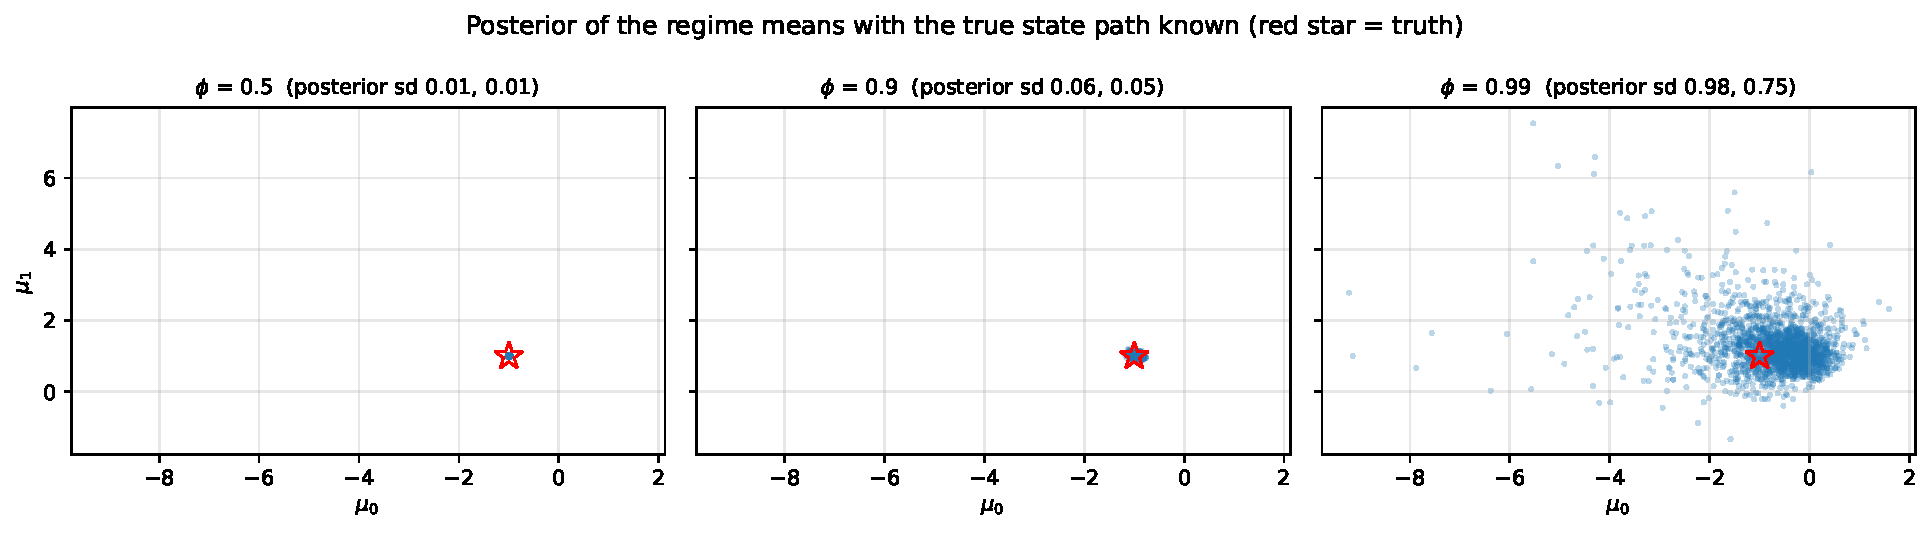
\includegraphics[width=0.9\textwidth]{regime_identification.pdf}
\vspace{-0.6cm}
\caption{Posterior draws of the regime means from data simulated with known regimes ($\mu_0=-1$, $\mu_1=1$, star) for
three persistence levels. At the persistence of the corn--soybean spread the means are not identified. \nb{06}}
\label{fig:regime}
\end{figure}

%=====================================================================
\section{Summary and lessons}\label{sec:lessons}
%=====================================================================
Table~\ref{tab:results} collects the out-of-sample results. The portfolio of pairs (E) is the only strategy that
performs consistently in training and test, and even its Sharpe ratio of about 0.4 over 4.4 years is within one
standard error of zero \citep{lo2002}. The machine-learning strategies are positive on their short holdouts, but with
standard errors near 0.9 and results that move with innocuous choices. All numbers ignore transaction costs. We
conclude that we did not find a robust corn--soybean (or grains) spread strategy. What we would tell the next team:

\begin{enumerate}
\item \textbf{Choose everything on training data.} In the first versions, entry thresholds and rolling windows were
picked after looking at the test sample, and the pairs portfolio was tuned on the full sample. Each looked like a
small shortcut, and each inflated the reported performance.
\item \textbf{Backtest tradeable P\&L.} Freeze the hedge at entry, keep units consistent (a log-price hedge ratio is
a ratio of \emph{dollar} positions, not of units), and divide by capital, not by the spread's standard deviation. The
earlier Sharpe ratio of 1.6 for the pairs portfolio was in spread-volatility units; with capital-normalised P\&L
and a proper split it is about 0.4.
\item \textbf{Overlapping labels are not independent.} Our very first ML backtest reported a Sharpe ratio of about 2 by
treating the P\&L of daily, heavily overlapping triple-barrier trades as a daily return series. Such labels need
uniqueness weights, purging and walk-forward validation to be evaluated honestly.
\item \textbf{In-sample cointegration is not a trading signal.} Use proper Engle--Granger critical values; and even
where the tests pass, they did not predict which spreads were profitable out of sample.
\item \textbf{Slow mean reversion means low power.} With half-lives of one to four months there are few independent
trades in a five-year test sample; a Sharpe ratio of 0.5 then has a standard error of about 0.45. After trying dozens of
specifications, the best test result is biased upwards.
\item \textbf{Know the data.} Continuous futures jump at rolls, early cotton ETF prices are stale, and one weather
location was downloaded with the wrong longitude sign.
\end{enumerate}
Natural next steps are longer histories of properly back-adjusted futures, explicit transaction costs, and
fundamental information (USDA supply estimates, planted acreage) rather than raw weather.

\bibliographystyle{plainnat}
{\small \bibliography{references}}

\end{document}
